\begin{frame}\frametitle{Strategy}
\centering\myskip

\begin{minipage}{.25\textwidth}\centering
\footnotesize

$$\TTbar\to WbWb$$ 
like $$\ttbar\to WbWb$$

\myskip
\myskip


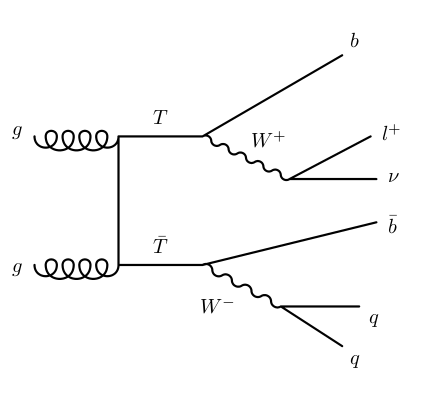
\includegraphics[width=1.15\textwidth]{pics/feyn_wbwb}


\end{minipage}\begin{minipage}{.75\textwidth}\centering
\vskip-5ex
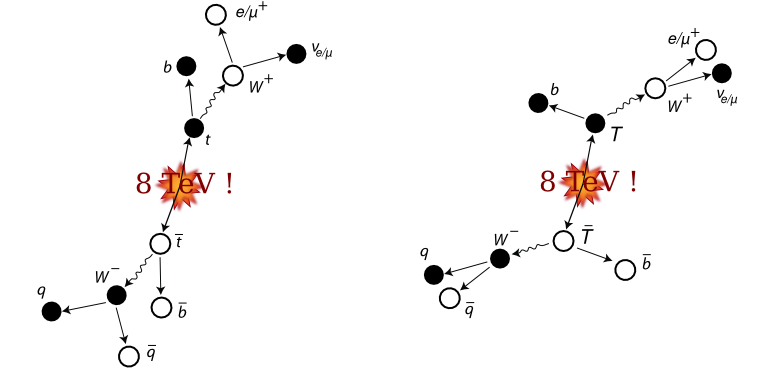
\includegraphics[width=1.\textwidth]{../wbx_analysis_14ifb/figures/kin.png}

different {\cccolor boosted kinematics}\\
{\LARGE $\Downarrow$}\\
reconstruct the $W$ boson from hadronic decay\\
{\LARGE $\swarrow\searrow$}\\
\begin{minipage}{.3\textwidth}\centering
merged jets\\
\wi
\end{minipage}\begin{minipage}{.3\textwidth}\centering
close-by jets\\
\wii
\end{minipage}

\end{minipage}

\end{frame}

%%%%%%%%%%%%%%%%%%%%%%%%%
%%%
%%%%%%%%%%%%%%%%%%%%%%%%%
\begin{frame}\frametitle{$W$ boson reconstruction}
\centering\footnotesize

\begin{minipage}{.34\textwidth}\centering

{\cccolor \large \wi}

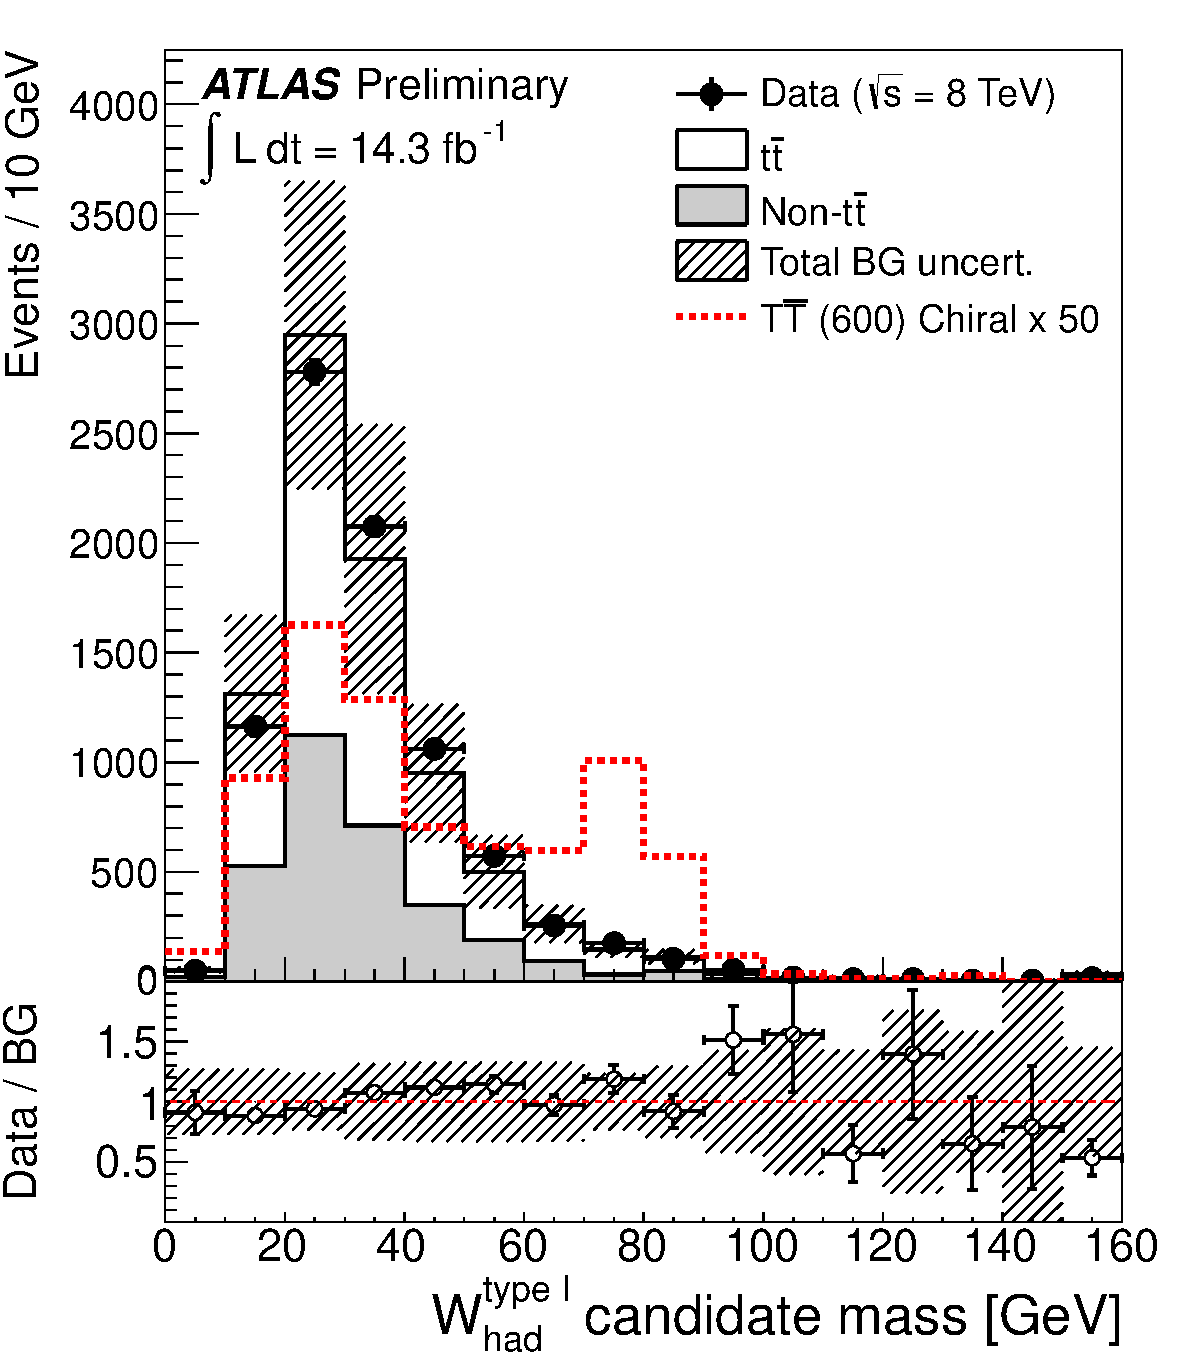
\includegraphics[width=1.\textwidth]{pics/VLQAna_WbX_WpreselType1_M_ELEMUON_preselW_NOMINAL}
\end{minipage}\begin{minipage}{.31\textwidth}\centering

%$$\Rightarrow$$
%$$\Leftarrow$$
{ \footnotesize
\myskip

\hskip-3ex
\begin{tabular}{p{.05cm} c}
%\toprule
\ldelim\{{5}{5ex}[] & \\
                      & one jet \\
                      & $\pt>250\gev$ \\
                      & $60<M<120\gev$ \\
& \\
\end{tabular}

\myskip

\hskip-3ex
\begin{tabular}{c p{.05cm}}
%\toprule
 & \rdelim\}{7}{7ex}[]\\
 no \wi & \\
 di-jet system &\\
 $\dr(j,j)<0.8$&  \\
 $\pt>200\gev$&  \\
 $60<M<120\gev$&  \\
& \\
\end{tabular}
}


\end{minipage}\begin{minipage}{.35\textwidth}\centering

{\cccolor \large \wii}

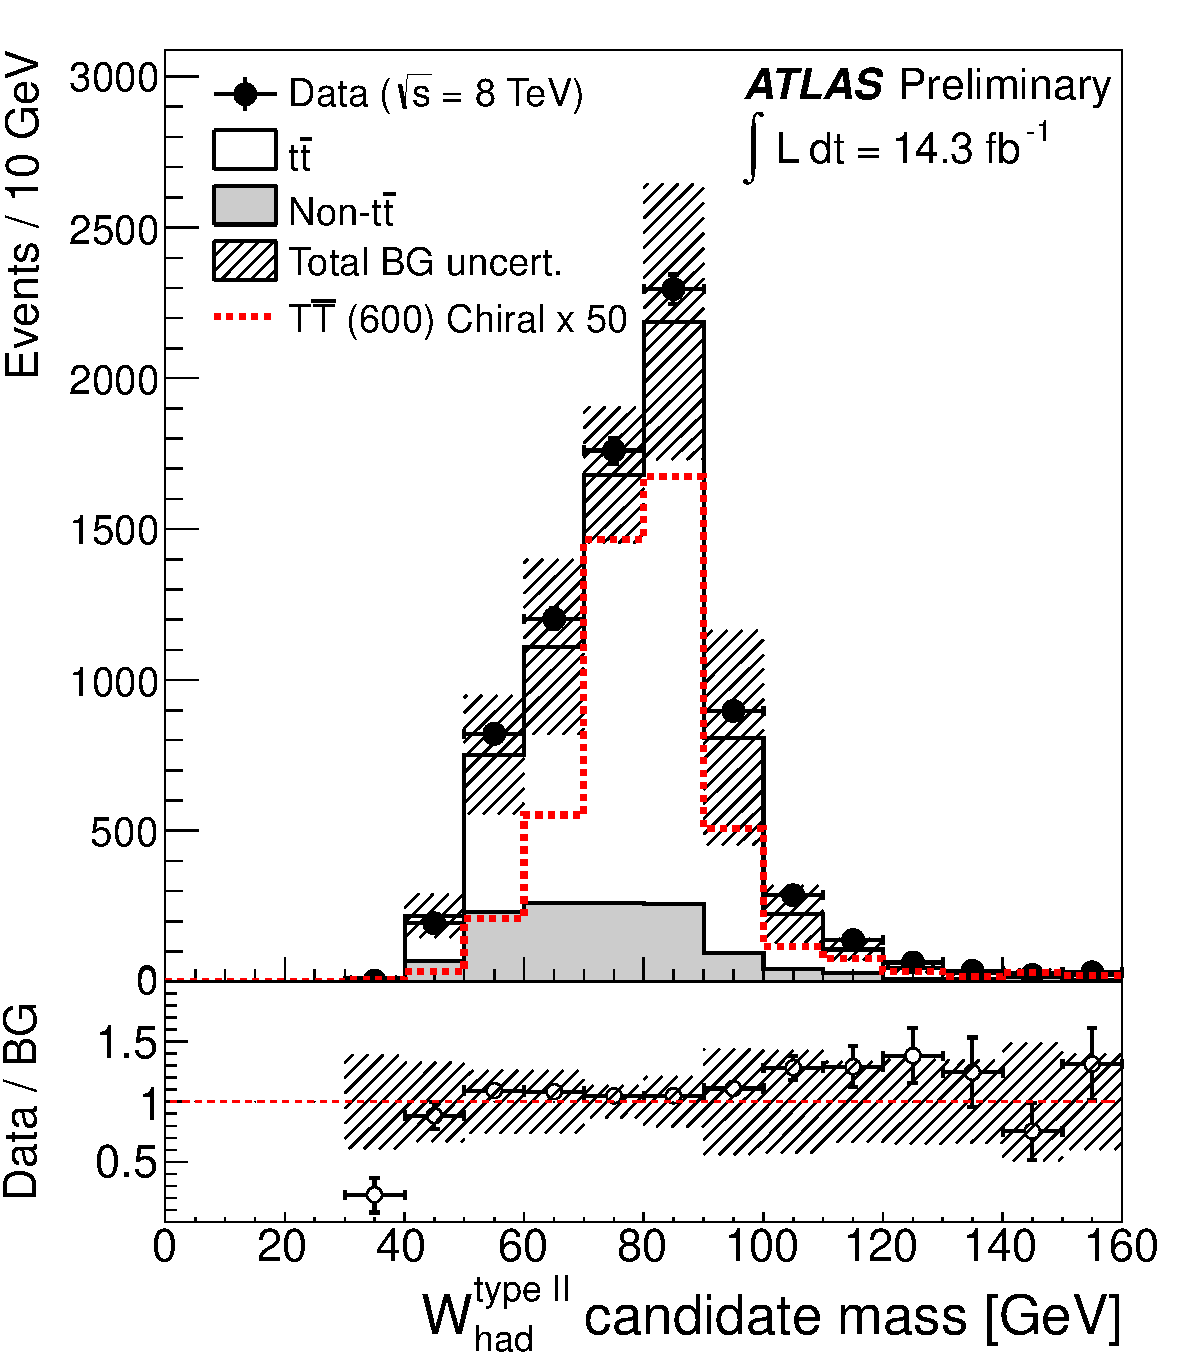
\includegraphics[width=1.\textwidth]{pics/VLQAna_WbX_WpreselType2_M_ELEMUON_preselW_NOMINAL}
\end{minipage}

\myskip

{\cccolor \wlep\ } reconstructed using {\cccolor lepton} and {\cccolor ``neutrino''}:\\
$p_X, p_Y$ from \met, $p_Z$ from $M_W^2 = (P_l + P_{\nu})^2$


\end{frame}

%%%%%%%%%%%%%%%%%%%%%%%%%
%%%
%%%%%%%%%%%%%%%%%%%%%%%%%
\begin{frame}\frametitle{Event selection}
\centering\footnotesize

\begin{minipage}{.5\textwidth}\centering
\begin{tabular}{ll}
\toprule
\multicolumn{2}{c}{\loose\ selection}\\
 SR0 & Preselection  \\
 SR1 & +\hskip5ex$\geq 1~W_{\rm had}$ candidates \\
 SR2 & +\hskip5ex$\htfj>800\gev$ \\
 SR3 & +\hskip5ex $\pt(b_1) > 160\gev$\\
 SR4 & +\hskip5ex$\pt(b_2) >80\gev$ \\
 SR5 & +\hskip5ex$\Delta R(\ell,\nu)<1.2$ \\
\bottomrule
\toprule
\multicolumn{2}{c}{\tight\  selection} \\
 SR5 & \loose\ selection \\
 SR6 &  +\hskip5ex min$\Delta R(\ell,b)>1.4$\\
 SR7 & +\hskip5ex min$\Delta R(W_{\rm had},b)>1.4$ \\
\bottomrule
\end{tabular}

%N.B. \bjet s are the two jets with highest \btag\ weight

\end{minipage}\begin{minipage}{.5\textwidth}\centering



\begin{pgfpicture}{0.0\textwidth}{0.0\textheight}{1.\textwidth}{.6\textwidth}
   \begin{pgftranslate}{\pgfpoint{0.05\textwidth}{-0.12\textheight}}
\pgfdeclareimage[interpolate=true,width=.95\textwidth]{htall}{pics/HTAll_ELEMUON_cutflow1_NOMINAL.pdf}
\pgfdeclareimage[interpolate=true,width=.95\textwidth]{jetptb1}{pics/JetPtB1_ELEMUON_cutflow12_NOMINAL.pdf}
\pgfdeclareimage[interpolate=true,width=.95\textwidth]{jetptb2}{pics/JetPtB2_ELEMUON_cutflow123_NOMINAL.pdf}
\pgfdeclareimage[interpolate=true,width=.95\textwidth]{nwhad}{pics/nWhad_ELEMUON_cutflow0_NOMINAL_logscale.pdf}
\pgfdeclareimage[interpolate=true,width=.95\textwidth]{mrecoT}{pics/VLQAna_WbX_1W_MWb_4_ELEMUON_cutflow1234567_NOMINAL.pdf}
\pgfdeclareimage[interpolate=true,width=.95\textwidth]{mrecoL}{pics/VLQAna_WbX_1W_MWb_4_ELEMUON_cutflow12345_NOMINAL.pdf}
\pgfdeclareimage[interpolate=true,width=.95\textwidth]{drlep}{pics/VLQAna_WbX_DRLepMet_ELEMUON_cutflow1234_NOMINAL.pdf}
\pgfdeclareimage[interpolate=true,width=.95\textwidth]{mindrl}{pics/VLQAna_WbX_MinDRlb_ELEMUON_cutflow12345_NOMINAL.pdf}
\pgfdeclareimage[interpolate=true,width=.95\textwidth]{mindrw}{pics/VLQAna_WbX_MinDRWb_ELEMUON_cutflow123456_NOMINAL.pdf}
%\pgfputat{\pgfxy(0.0,0.0)}{\pgfbox[left,base]{\pgfuseimage{mindr}}}
 \pgfsetlinewidth{1.pt}
 \usebeamercolor[bg]{head/foot boxes}
\only<1>{
 \pgfrect[stroke]{\pgfxy(-6,3.82)}{\pgfxy(5,0.35)}
 %\pgfline{\pgfxy(1.55,1.5)}{\pgfxy(1.55,3.5)} 
 \pgfstroke
\pgfputat{\pgfxy(0.0,-0.8)}{\pgfbox[left,base]{\pgfuseimage{nwhad}}}
}
\only<2>{
 \pgfrect[stroke]{\pgfxy(-6,3.46)}{\pgfxy(5,0.35)}
 %\pgfline{\pgfxy(1.55,1.5)}{\pgfxy(1.55,3.5)} 
 \pgfstroke
\pgfputat{\pgfxy(0.0,-0.8)}{\pgfbox[left,base]{\pgfuseimage{htall}}}
}
\only<3>{
 \pgfrect[stroke]{\pgfxy(-6,3.1)}{\pgfxy(5,0.35)}
 %\pgfline{\pgfxy(1.55,1.5)}{\pgfxy(1.55,3.5)} 
 \pgfstroke
\pgfputat{\pgfxy(0.0,-0.8)}{\pgfbox[left,base]{\pgfuseimage{jetptb1}}}
}
\only<4>{
 \pgfrect[stroke]{\pgfxy(-6,2.74)}{\pgfxy(5,0.35)}
 %\pgfline{\pgfxy(1.55,1.5)}{\pgfxy(1.55,3.5)} 
 \pgfstroke
\pgfputat{\pgfxy(0.0,-0.8)}{\pgfbox[left,base]{\pgfuseimage{jetptb2}}}
}
\only<5>{
 \pgfrect[stroke]{\pgfxy(-6,2.45)}{\pgfxy(5,0.35)}
 %\pgfline{\pgfxy(1.55,1.5)}{\pgfxy(1.55,3.5)} 
 \pgfstroke
\pgfputat{\pgfxy(0.0,-0.8)}{\pgfbox[left,base]{\pgfuseimage{drlep}}}
}
\only<6>{
 \pgfrect[stroke]{\pgfxy(-6,1.15)}{\pgfxy(5,0.35)}
 %\pgfline{\pgfxy(1.55,1.5)}{\pgfxy(1.55,3.5)} 
 \pgfstroke
\pgfputat{\pgfxy(0.0,-0.8)}{\pgfbox[left,base]{\pgfuseimage{mindrl}}}
}
\only<7>{
 \pgfrect[stroke]{\pgfxy(-6,0.8)}{\pgfxy(5,0.35)}
 %\pgfline{\pgfxy(1.55,1.5)}{\pgfxy(1.55,3.5)} 
 \pgfstroke
\pgfputat{\pgfxy(0.0,-0.8)}{\pgfbox[left,base]{\pgfuseimage{mindrw}}}
}
   \end{pgftranslate}

\end{pgfpicture}

\end{minipage}

\end{frame}


%%%%%%%%%%%%%%%%%%%%%%%%%
%%%
%%%%%%%%%%%%%%%%%%%%%%%%%
\begin{frame}\frametitle{Comparison data vs prediction}
\centering\footnotesize

\begin{minipage}{.5\textwidth}\centering

Check agreement between data and background prediction

{\Large$\Downarrow$}

Define regions depleted in signal

\myskip

\scriptsize
\begin{tabular}{l*{1}{r@{ $\pm$ }r@{ }l}}
\toprule
 & \multicolumn{3}{c}{\loose\ but $\Delta R(\ell,\nu)>1.2$}\\
\midrule
$t\bar{t'} (600\GeV)$ & $18.47$ & $1.48$ & $^{+1.09}_{-1.64}$\\
\midrule
$t\bar{t}$ & $173.13$ & $8.82$ & $^{+46.92}_{-48.59}$\\
$W$+jets & $30.64$ & $9.78$ & $^{+13.74}_{-12.43}$\\
$Z$+jets & $11.68$ & $5.93$ & $^{+5.89}_{-6.96}$\\
Diboson & $0.29$ & $0.19$ & $^{+0.17}_{-0.17}$\\
Single top & $21.46$ & $2.54$ & $^{+2.60}_{-2.54}$\\
$t\bar{t}$$V$ & $4.21$ & $0.16$ & $^{+1.33}_{-1.33}$\\
Multijet & $0.49$ & $0.91$ & $ \pm\ 0.25$\\
\midrule
Total bkg. & $241.90 $ & $ 14.70$ & $ ^{+53.57}_{-55.95}$\\
\midrule
Data & \multicolumn{3}{c}{$250$}\\
\bottomrule
\end{tabular}


\end{minipage}\begin{minipage}{.5\textwidth}\centering

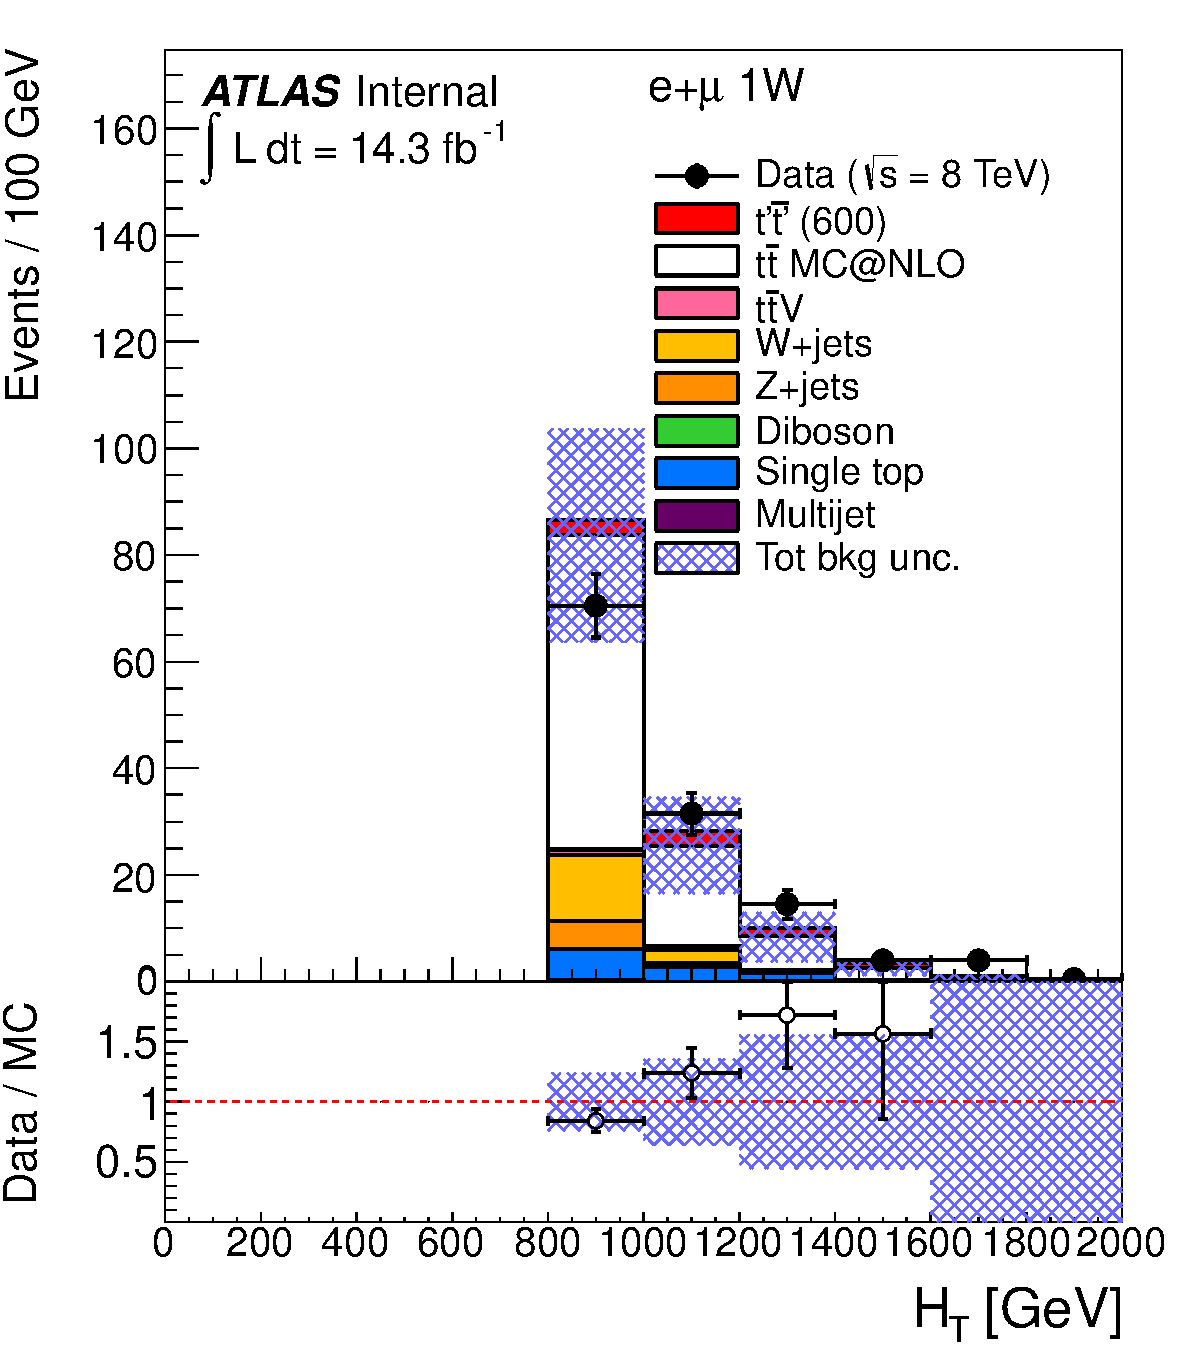
\includegraphics[width=.5\textwidth]{pics/HTAll_ELEMUONCR3_1W_NOMINAL.pdf}
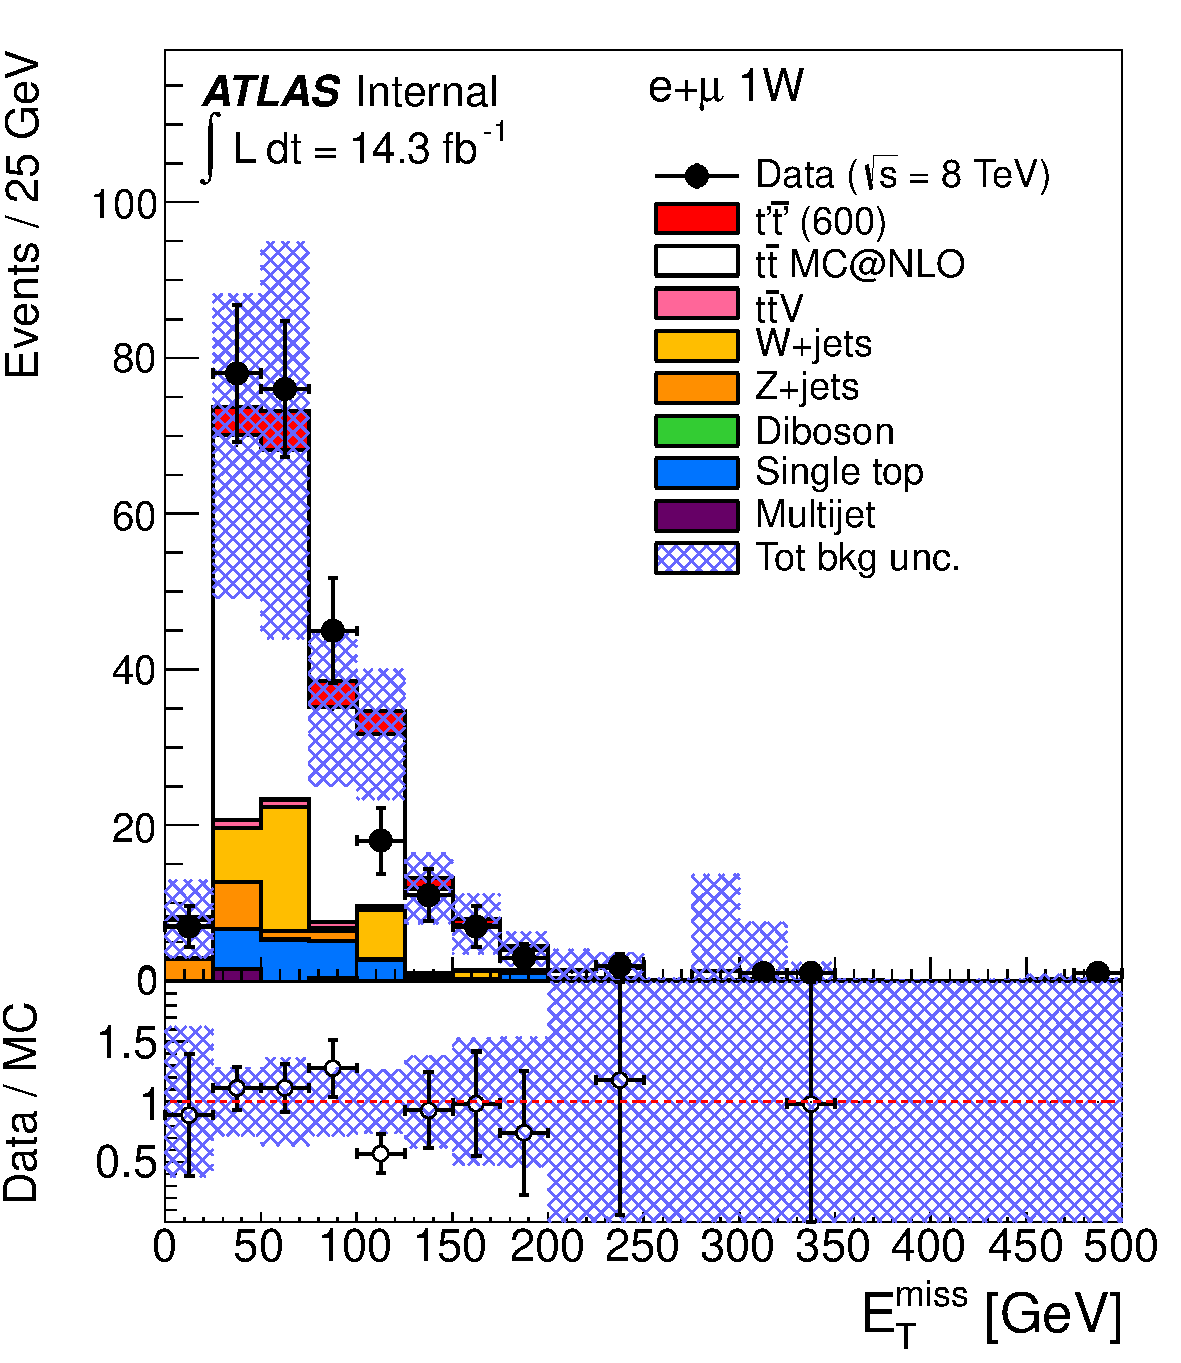
\includegraphics[width=.5\textwidth]{pics/MET_ELEMUONCR3_1W_NOMINAL.pdf}\\
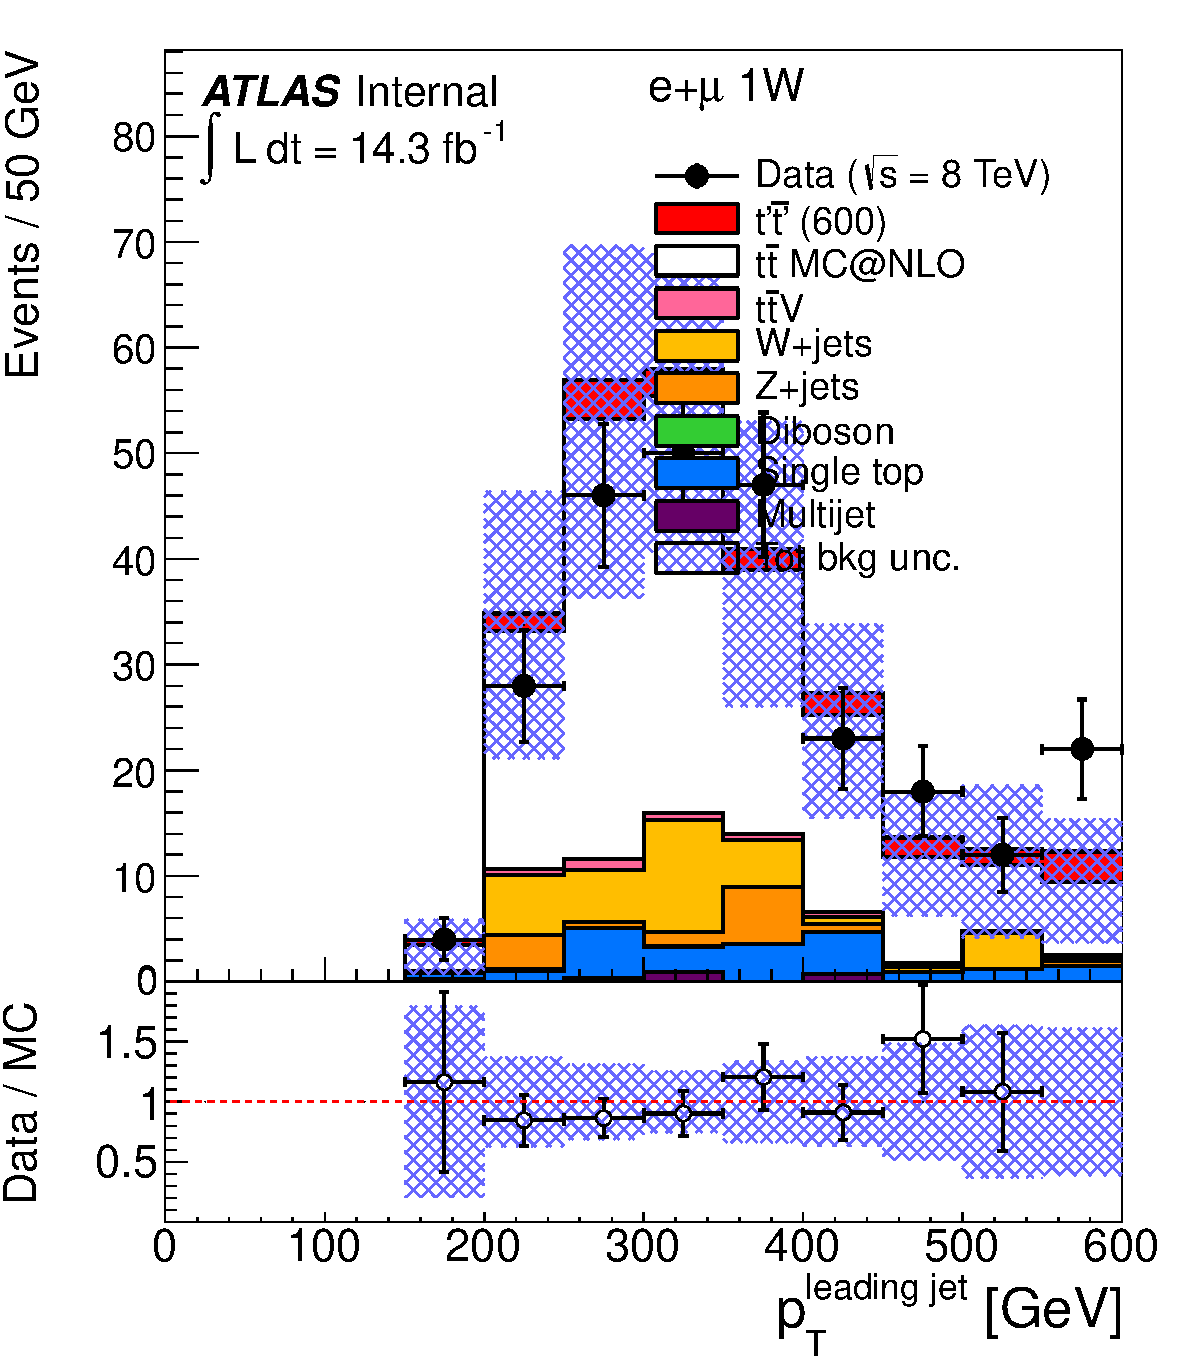
\includegraphics[width=.5\textwidth]{pics/JetPt1_ELEMUONCR3_1W_NOMINAL.pdf}
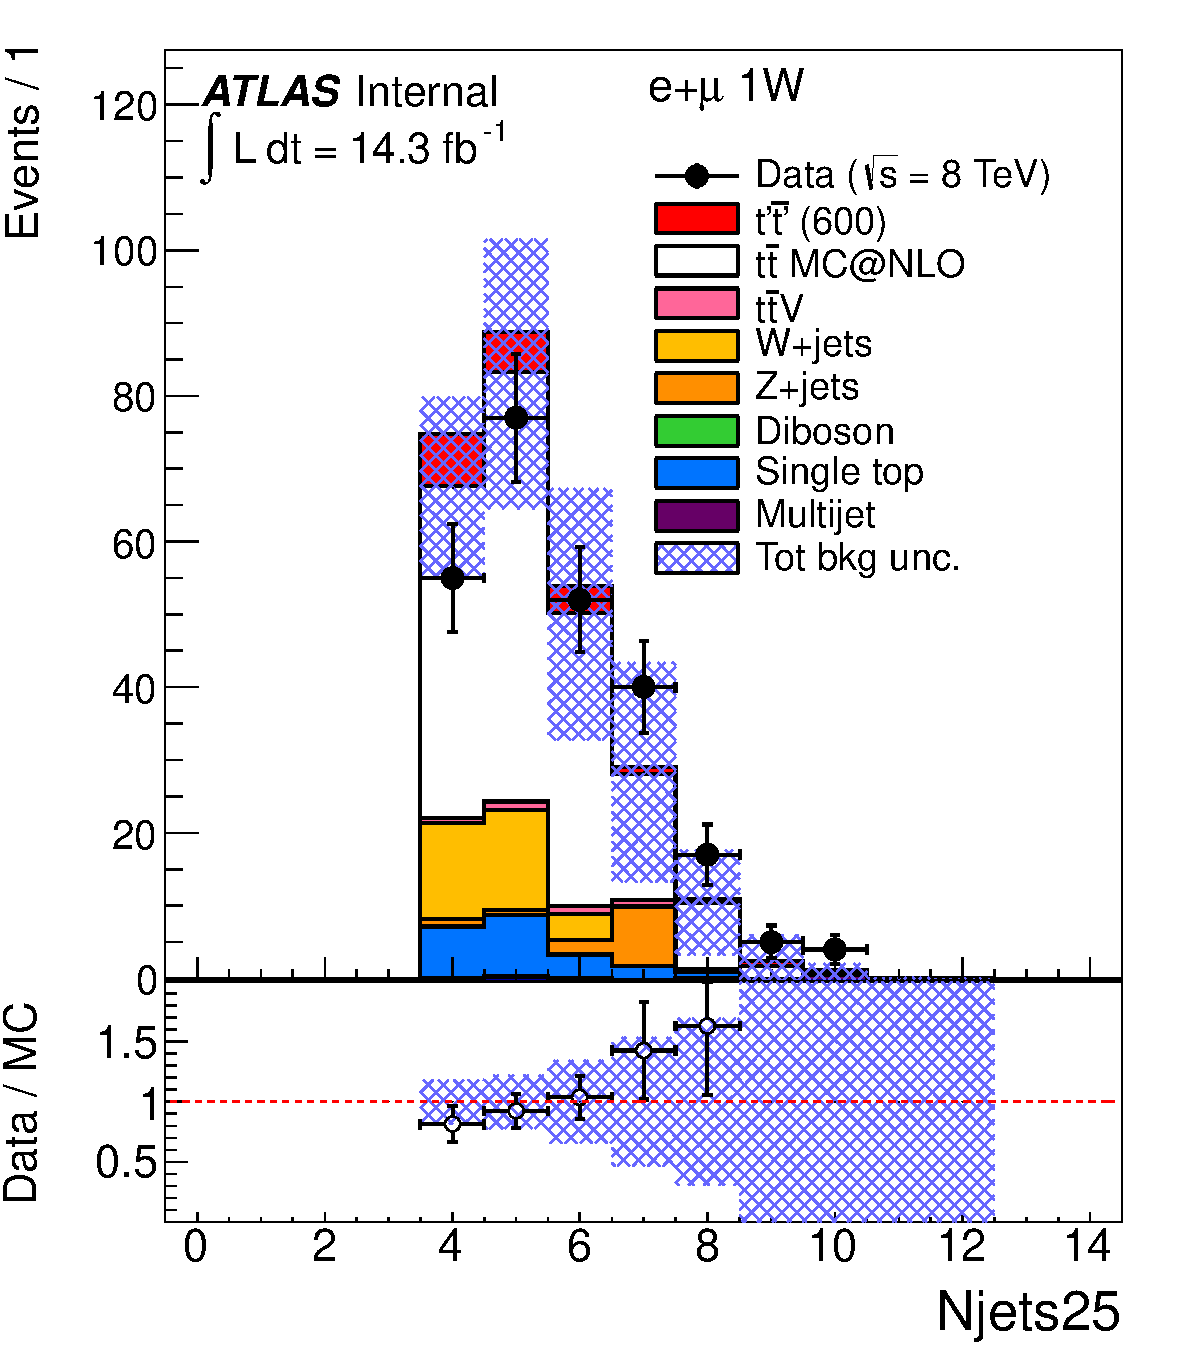
\includegraphics[width=.5\textwidth]{pics/Njets25_ELEMUONCR3_1W_NOMINAL.pdf}

\end{minipage}

\end{frame}


%%%%%%%%%%%%%%%%%%%%%%%%%
%%%
%%%%%%%%%%%%%%%%%%%%%%%%%
\begin{frame}\frametitle{Yields in signal region}
\centering\scriptsize

\begin{minipage}{.6\textwidth}\centering

\hskip-5ex
\begin{tabular}{p{0.05cm} p{0.05cm}}
\\
\\
%\parbox[t]{2mm}{\multirow{5}{*}{\rotatebox[origin=c]{90}{rota}}}& \ldelim\{{5}{5ex} \\
\multirow{5}{*}{\rotatebox[origin=c]{90}{\cccolor merged}}& \ldelim\{{5}{5ex} \\
\\
\\
\\
\\
\\
\\
\\
\\
\\
\\
\end{tabular}\begin{tabular}{l  D{;}{\,\pm\,}{-1} D{;}{\,\pm\,}{-1} }
    \toprule
    & \multicolumn{1}{c}{\loose} 
    & \multicolumn{1}{c}{\tight}  \\\midrule
$t\bar{t}$    & 264;80 & 10;6 \\
$t\bar{t}V$   &  5.1;1.8 & 0.5;0.2 \\
$W$+jets   &  16;11 & 6;5\\
$Z$+jets   &  1.1;1.4 & 0.2;0.5 \\
Single top   &  30;7 & 4.4;1.6  \\
Dibosons &  0.21;0.15 & 0.06;0.05 \\
\midrule
Tot.Bkg.  & 317;90 & 21;9 \\
Data& 348 & 37  \\
%Data& \multicolumn{1}{c}{348\,\phantom{$\pm$}} & 37  \\
\midrule
$T\bar{T}(600\GeV)$ \\
Chiral $t'$&  88;10 & 54;7 \\
$T$ Singlet      & 41;4 & 20.3;2.2 \\
\bottomrule\end{tabular}

\myskip

\footnotesize
Discriminating variable $\Rightarrow$ {\cccolor $T$ reconstructed mass}\\
{\large$\Downarrow$}\\
Pair \bjet s and $W$ boson candidates in order to get\\
min$\Delta(M_{\rm lep},M_{\rm had})$

\end{minipage}\begin{minipage}{.4\textwidth}\centering

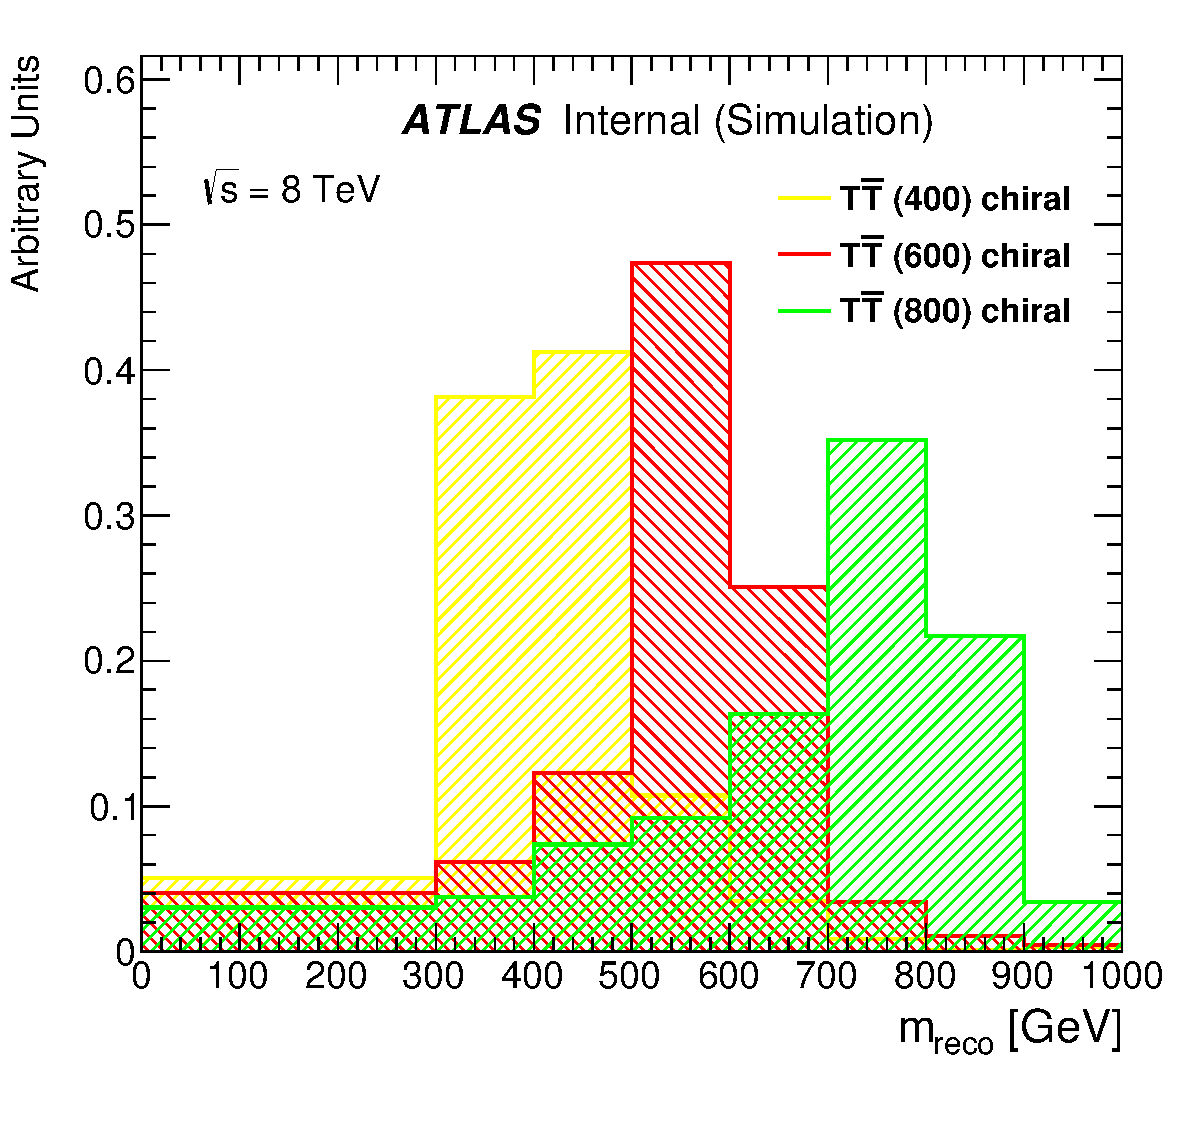
\includegraphics[width=.8\textwidth]{pics/VLQAna_WbX_1W_MWb_4_ELEMUONloose_1W_NOMINAL_VLTtt.pdf}\\
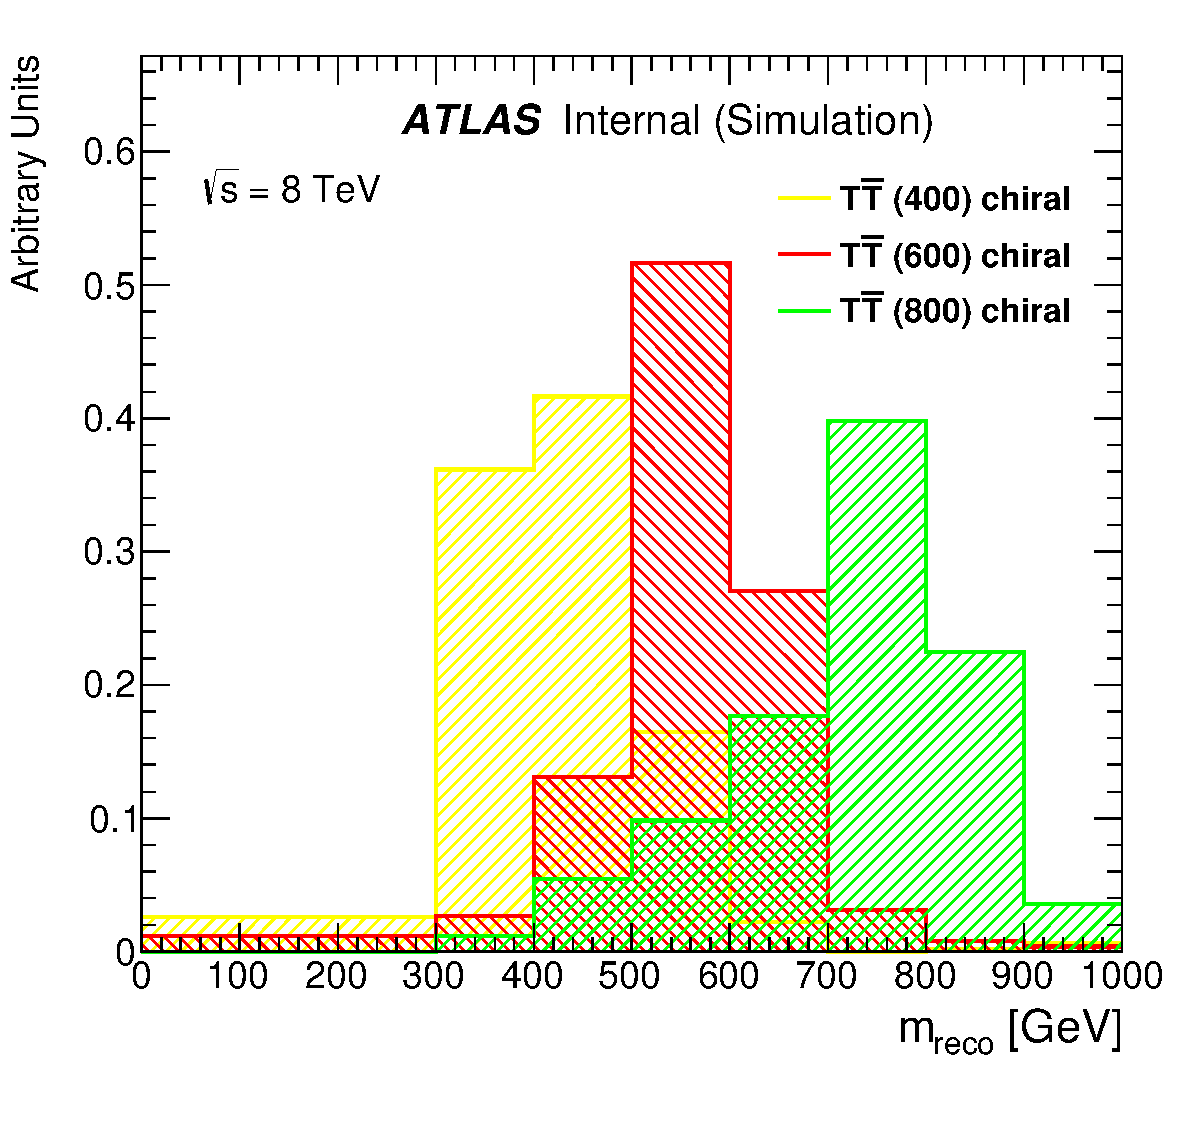
\includegraphics[width=.8\textwidth]{pics/VLQAna_WbX_1W_MWb_4_ELEMUONtight_1W_NOMINAL_VLTtt.pdf}
\end{minipage}

\end{frame}



%%%%%%%%%%%%%%%%%%%%%%%%%
%%%
%%%%%%%%%%%%%%%%%%%%%%%%%
\begin{frame}\frametitle{Reconstructed mass}
\centering\footnotesize

\begin{minipage}{.5\textwidth}\centering
\begin{tabular}{ll}
\toprule
\multicolumn{2}{c}{\loose\ selection}\\
 SR0 & Preselection  \\
 SR1 & +\hskip5ex$\geq 1~W_{\rm had}$ candidates \\
 SR2 & +\hskip5ex$\htfj>800\gev$ \\
 SR3 & +\hskip5ex $\pt(b_1) > 160\gev$\\
 SR4 & +\hskip5ex$\pt(b_2) >80\gev$ \\
 SR5 & +\hskip5ex$\Delta R(\ell,\nu)<1.2$ \\
\bottomrule
\toprule
\multicolumn{2}{c}{\tight\  selection} \\
 SR5 & \loose\ selection \\
 SR6 &  +\hskip5ex min$\Delta R(\ell,b)>1.4$\\
 SR7 & +\hskip5ex min$\Delta R(W_{\rm had},b)>1.4$ \\
\bottomrule
\end{tabular}

%N.B. \bjet s are the two jets with highest \btag\ weight

\end{minipage}\begin{minipage}{.5\textwidth}\centering



\begin{pgfpicture}{0.0\textwidth}{0.0\textheight}{1.\textwidth}{.6\textwidth}
   \begin{pgftranslate}{\pgfpoint{0.05\textwidth}{-0.12\textheight}}

\pgfdeclareimage[interpolate=true,width=.95\textwidth]{mreco6}{pics/THESIS_c6_cutflow/VLQAna_WbX_1W_MWb_4_ELEMUON_cutflow123456_NOMINAL.pdf}
\pgfdeclareimage[interpolate=true,width=.95\textwidth]{mreco4}{pics/THESIS_c6_cutflow/VLQAna_WbX_1W_MWb_4_ELEMUON_cutflow1234_NOMINAL.pdf}
\pgfdeclareimage[interpolate=true,width=.95\textwidth]{mreco3}{pics/THESIS_c6_cutflow/VLQAna_WbX_1W_MWb_4_ELEMUON_cutflow123_NOMINAL.pdf}
\pgfdeclareimage[interpolate=true,width=.95\textwidth]{mreco2}{pics/THESIS_c6_cutflow/VLQAna_WbX_1W_MWb_4_ELEMUON_cutflow12_NOMINAL.pdf}
\pgfdeclareimage[interpolate=true,width=.95\textwidth]{mreco1}{pics/THESIS_c6_cutflow/VLQAna_WbX_1W_MWb_4_ELEMUON_cutflow1_NOMINAL.pdf}
\pgfdeclareimage[interpolate=true,width=.95\textwidth]{mrecoT}{pics/VLQAna_WbX_1W_MWb_4_ELEMUON_cutflow1234567_NOMINAL.pdf}
\pgfdeclareimage[interpolate=true,width=.95\textwidth]{mrecoL}{pics/VLQAna_WbX_1W_MWb_4_ELEMUON_cutflow12345_NOMINAL.pdf}
%\pgfputat{\pgfxy(0.0,0.0)}{\pgfbox[left,base]{\pgfuseimage{mindr}}}
 \pgfsetlinewidth{1.pt}
 \usebeamercolor[bg]{head/foot boxes}
\only<1>{
 \pgfrect[stroke]{\pgfxy(-6,3.82)}{\pgfxy(5,0.35)}
 %\pgfline{\pgfxy(1.55,1.5)}{\pgfxy(1.55,3.5)} 
 \pgfstroke
\pgfputat{\pgfxy(0.0,-0.8)}{\pgfbox[left,base]{\pgfuseimage{mreco1}}}
}
\only<2>{
 \pgfrect[stroke]{\pgfxy(-6,3.46)}{\pgfxy(5,0.35)}
 %\pgfline{\pgfxy(1.55,1.5)}{\pgfxy(1.55,3.5)} 
 \pgfstroke
\pgfputat{\pgfxy(0.0,-0.8)}{\pgfbox[left,base]{\pgfuseimage{mreco2}}}
}
\only<3>{
 \pgfrect[stroke]{\pgfxy(-6,3.1)}{\pgfxy(5,0.35)}
 %\pgfline{\pgfxy(1.55,1.5)}{\pgfxy(1.55,3.5)} 
 \pgfstroke
\pgfputat{\pgfxy(0.0,-0.8)}{\pgfbox[left,base]{\pgfuseimage{mreco3}}}
}
\only<4>{
 \pgfrect[stroke]{\pgfxy(-6,2.74)}{\pgfxy(5,0.35)}
 %\pgfline{\pgfxy(1.55,1.5)}{\pgfxy(1.55,3.5)} 
 \pgfstroke
\pgfputat{\pgfxy(0.0,-0.8)}{\pgfbox[left,base]{\pgfuseimage{mreco4}}}
}
\only<5>{
 \pgfrect[stroke]{\pgfxy(-6,2.45)}{\pgfxy(5,0.35)}
 %\pgfline{\pgfxy(1.55,1.5)}{\pgfxy(1.55,3.5)} 
 \pgfstroke
\pgfputat{\pgfxy(0.0,-0.8)}{\pgfbox[left,base]{\pgfuseimage{mrecoL}}}
}
\only<6>{
 \pgfrect[stroke]{\pgfxy(-6,1.15)}{\pgfxy(5,0.35)}
 %\pgfline{\pgfxy(1.55,1.5)}{\pgfxy(1.55,3.5)} 
 \pgfstroke
\pgfputat{\pgfxy(0.0,-0.8)}{\pgfbox[left,base]{\pgfuseimage{mreco6}}}
}
\only<7>{
 \pgfrect[stroke]{\pgfxy(-6,0.8)}{\pgfxy(5,0.35)}
 %\pgfline{\pgfxy(1.55,1.5)}{\pgfxy(1.55,3.5)} 
 \pgfstroke
\pgfputat{\pgfxy(0.0,-0.8)}{\pgfbox[left,base]{\pgfuseimage{mrecoT}}}
}
   \end{pgftranslate}

\end{pgfpicture}

\end{minipage}

\end{frame}


%%%%%%%%%%%%%%%%%%%%%%%%%
%%%
%%%%%%%%%%%%%%%%%%%%%%%%%
\begin{frame}\frametitle{Most relevant systematic uncertainties}
\centering\footnotesize

\begin{tabular}{l*{3}{c}}
\toprule
 & $\T\bar{\T}$ ($600\gev$) & $t\bar{t}$ & Non-$t\bar{t}$\\
\midrule
Total [\%] & +14/-15 & +59/-59 & +42/-35\\
\midrule
Main contributions [\%] &&&\\
Jet energy scale & +6.6/-8.4 & +15/-15 & +33/-22\\  
$t\bar{t}$ modelling: NLO MC generator & -- & +48/-48 & --\\  
$t\bar{t}$ modelling: PS and fragm & -- & +25/-25 & --\\  
$t\bar{t}$ modelling: ISR/FSR & -- & +8.8/-8.8 & --\\   
\bottomrule
\end{tabular}

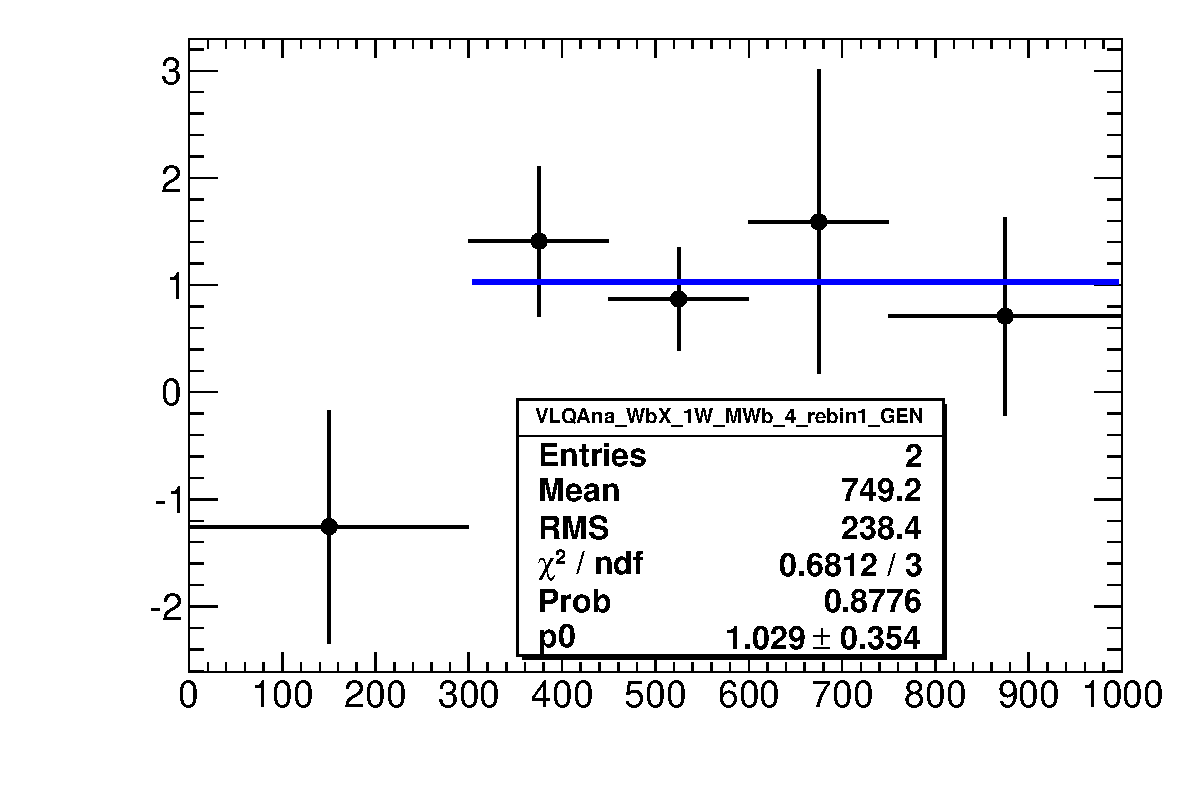
\includegraphics[width=.33\textwidth]{pics/GEN_RATIO.pdf}
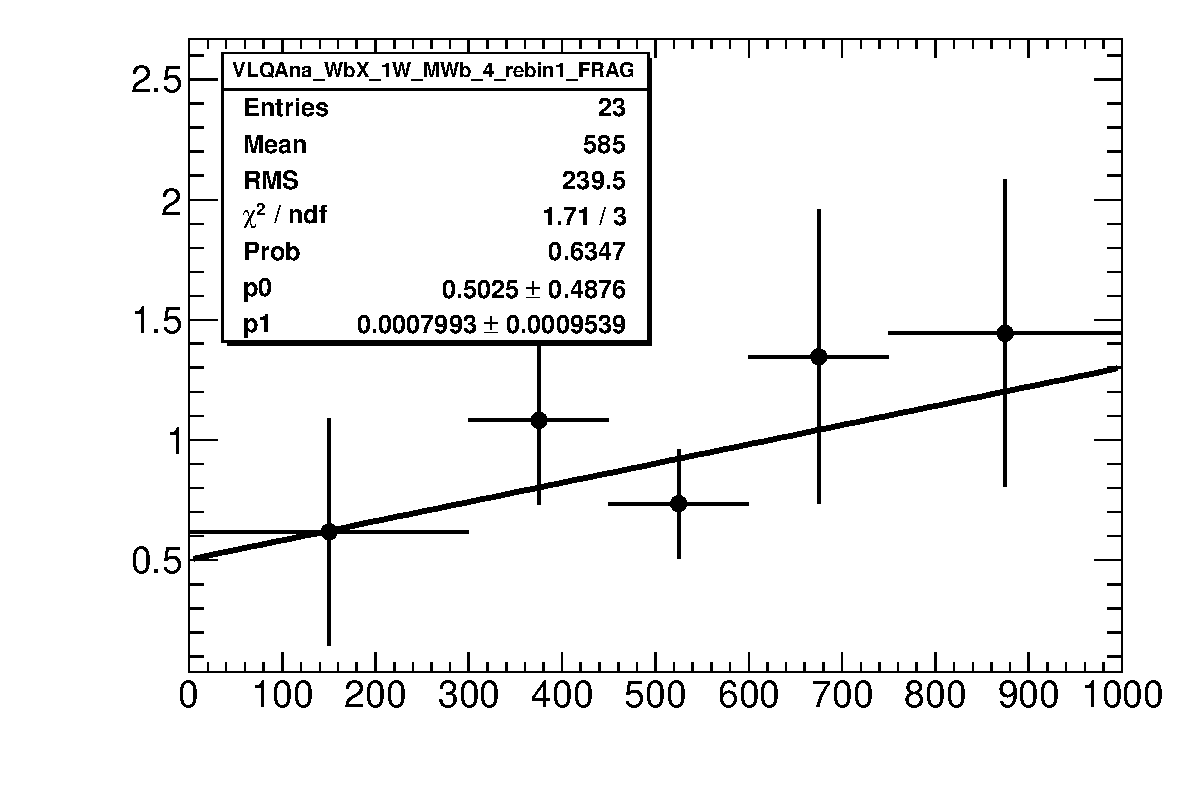
\includegraphics[width=.33\textwidth]{pics/FRAG_RATIO.pdf}
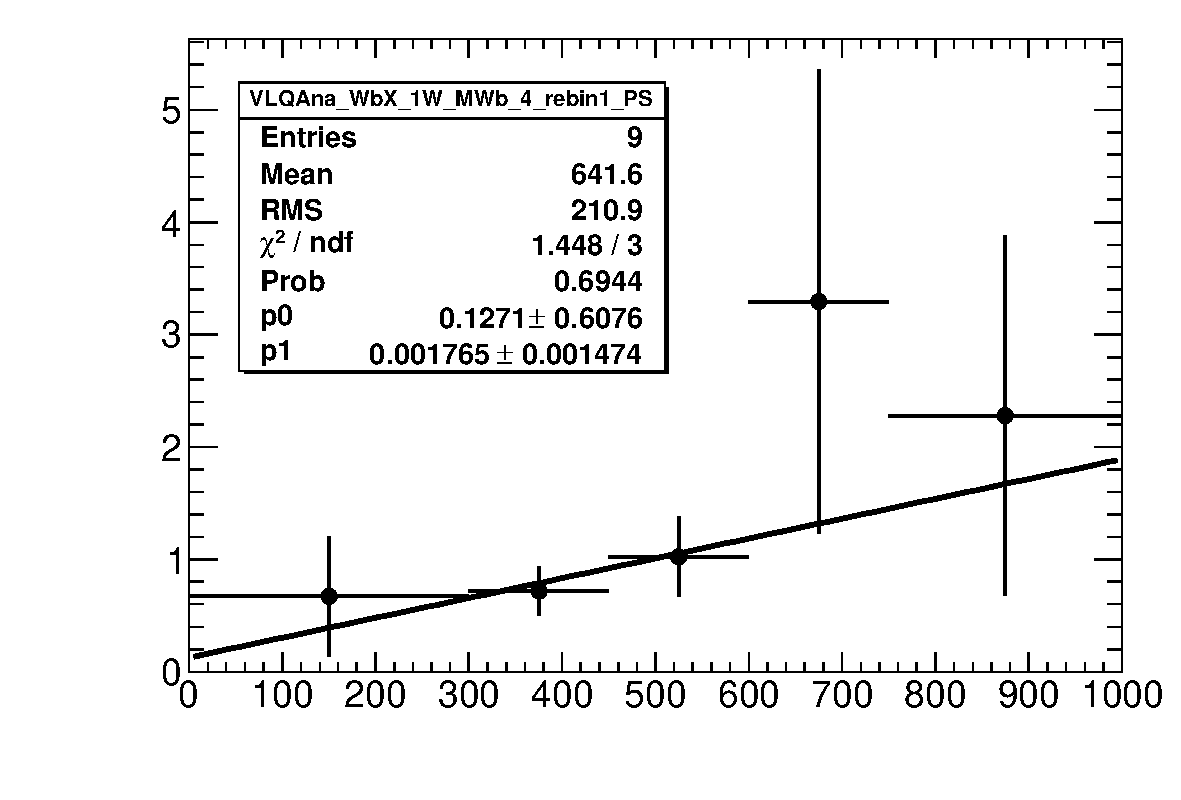
\includegraphics[width=.33\textwidth]{pics/PS_RATIO.pdf}

\end{frame}

%%%%%%%%%%%%%%%%%%%%%%%%%
%%%
%%%%%%%%%%%%%%%%%%%%%%%%%
\begin{frame}\frametitle{Results}
\centering\footnotesize

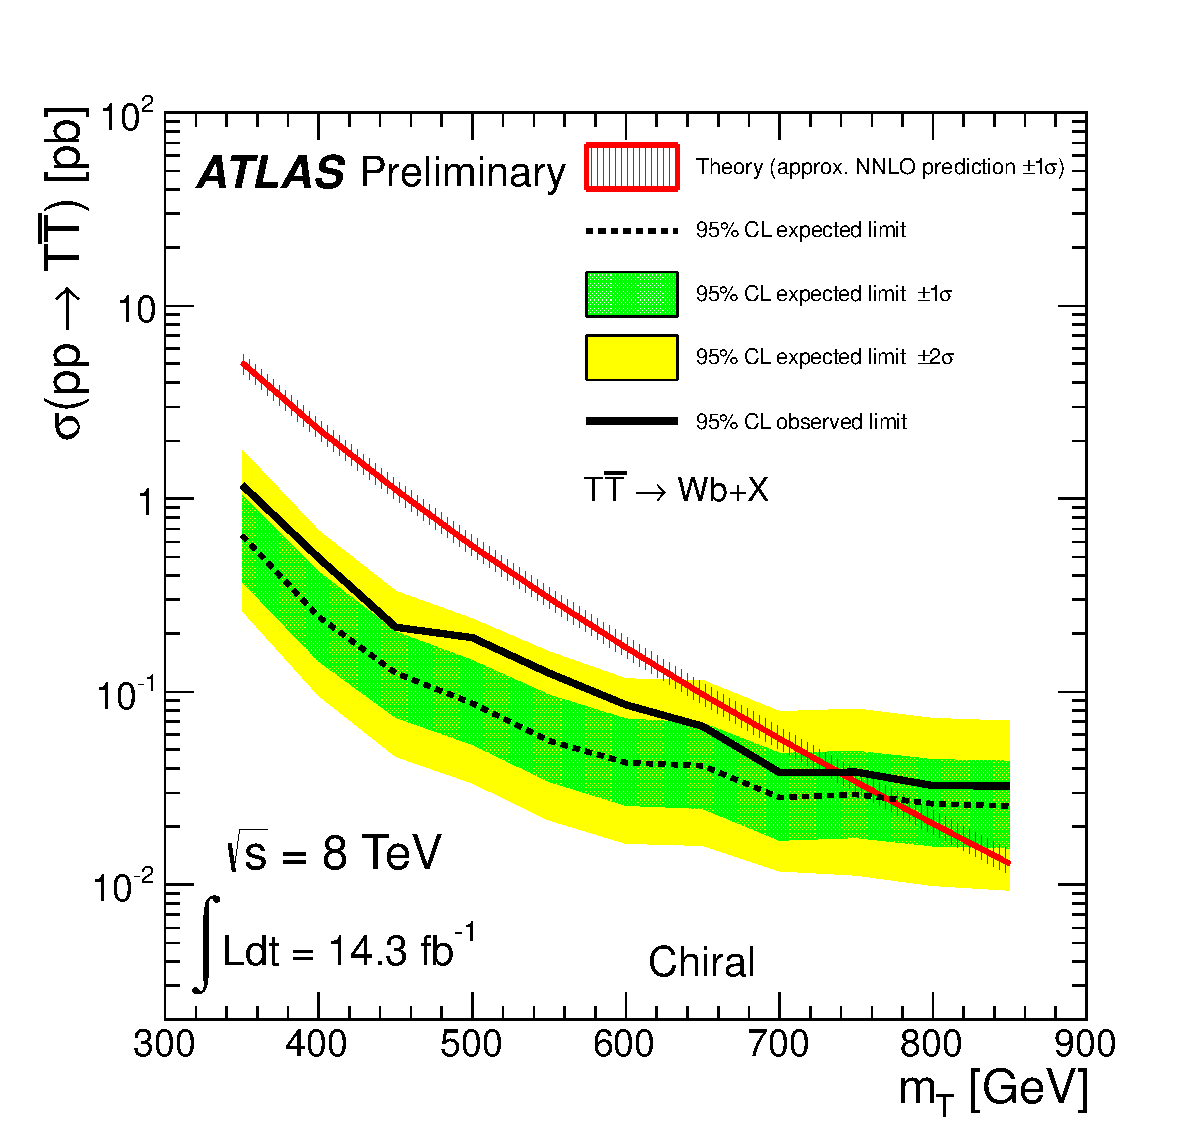
\includegraphics[width=0.45\textwidth]{pics/lim_chiral_bin1_WbX}
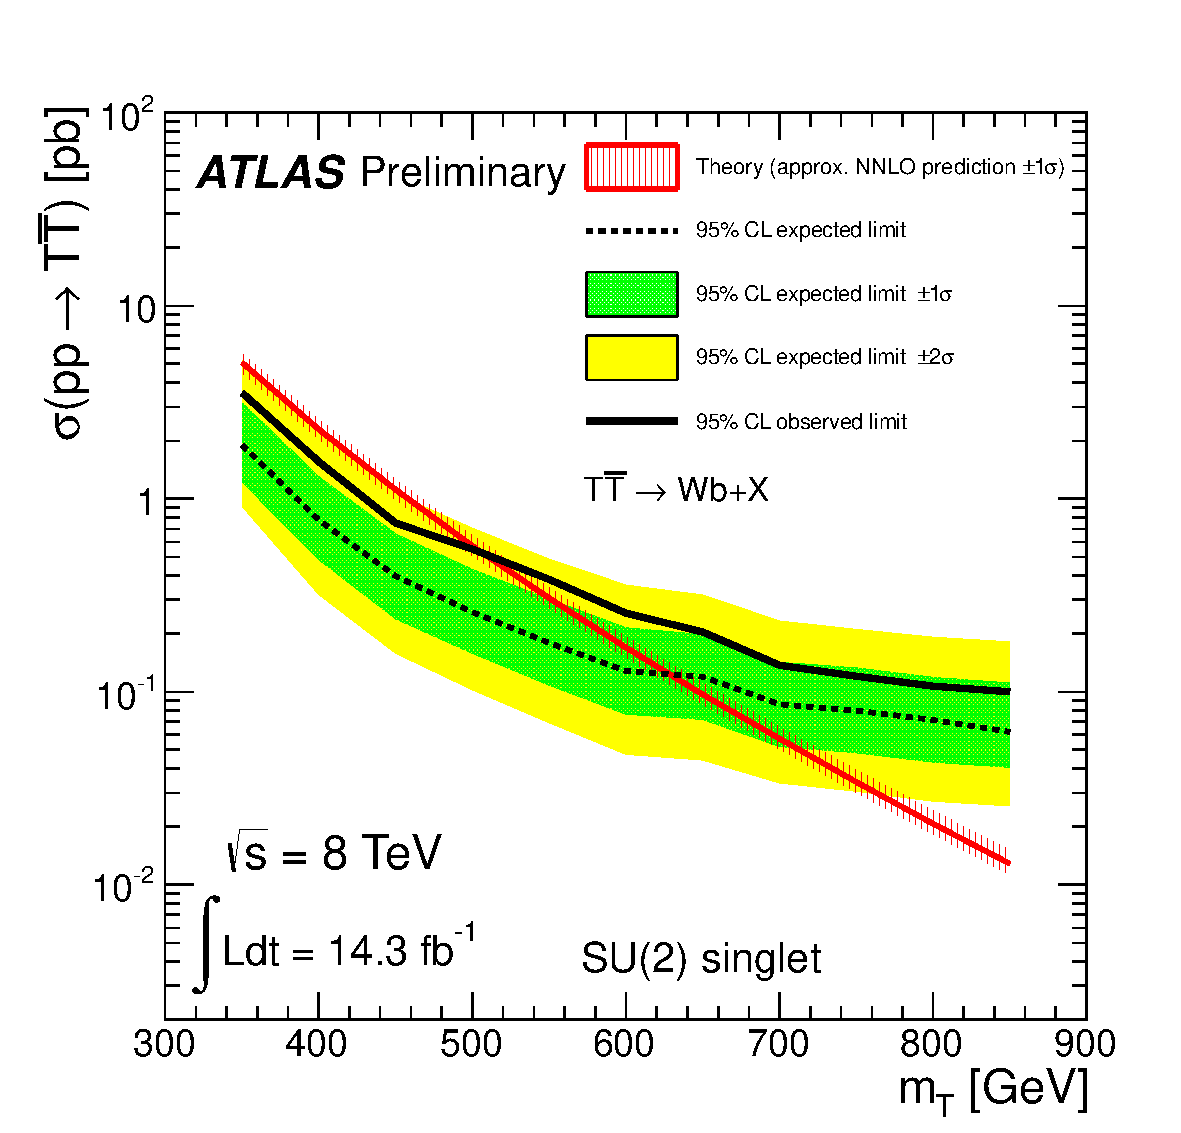
\includegraphics[width=0.45\textwidth]{pics/lim_singlet_bin1_WbX}


\end{frame}

%%%%%%%%%%%%%%%%%%%%%%%%%
%%%
%%%%%%%%%%%%%%%%%%%%%%%%%
\begin{frame}\frametitle{Results}
\centering\footnotesize

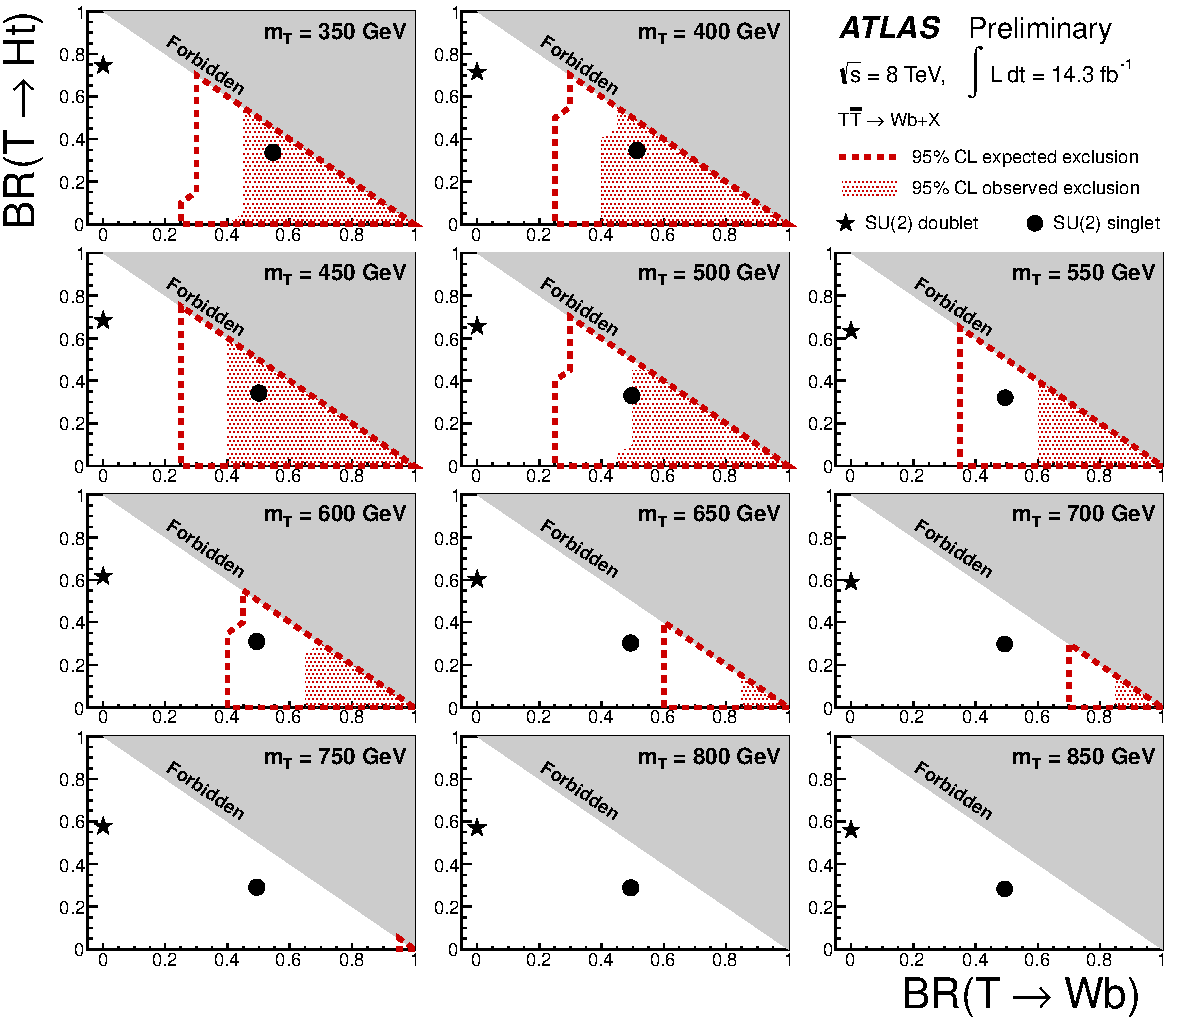
\includegraphics[width=0.7\textwidth]{pics/lim_Scan2D_tight_Bin1.pdf}

\end{frame}



